\documentclass{abnt}

%Arquivo com os principais pacotes usados e suas descrições.

%%%%%%%%%%%%%%%%%%%%%%%%%%%%%%%%%%%%%%%%%
% 			Idiomas e Acentos			%
%%%%%%%%%%%%%%%%%%%%%%%%%%%%%%%%%%%%%%%%%
\usepackage[brazilian]{babel} % Habilita o uso do idioma português do brasil (PT-BR).
\usepackage[T1]{fontenc} 
%\usepackage{fontspec} % Habilita maior variedade de acentos. Pode ser necessario adicionar outros pacotes.
\usepackage{lmodern} % Habilita o uso da font Latin Modern.


%%%%%%%%%%%%%%%%%%%%%%%%%%%%%%%%%%%%%%%%%
% 				TABELAS					%
%%%%%%%%%%%%%%%%%%%%%%%%%%%%%%%%%%%%%%%%%
\usepackage{tabulary} % Cria tabelas mais facilmente.
\usepackage{booktabs} % Melhora o visual das tabelas.
\usepackage[table]{xcolor} % Pacote de cor pra as tabelas.
\usepackage{caption} % Melhora as legendas de imagens, tabela etc.

%%%%%%%%%%%%%%%%%%%%%%%%%%%%%%%%%%%%%%%%%
% 				IMAGENS					%
%%%%%%%%%%%%%%%%%%%%%%%%%%%%%%%%%%%%%%%%%
\usepackage{graphicx} % Facilita a inserção de imagens.


%%%%%%%%%%%%%%%%%%%%%%%%%%%%%%%%%%%%%%%%%
% 			CÓDIGO FONTE				%
%%%%%%%%%%%%%%%%%%%%%%%%%%%%%%%%%%%%%%%%%

%Documentação de código fonte.
\usepackage{listings}


%%%%%%%%%%%%%%%%%%%%%%%%%%%%%%%%%%%%%%%%%
% 	Símbolos e Caracteres Matemáticos	%
%%%%%%%%%%%%%%%%%%%%%%%%%%%%%%%%%%%%%%%%%
\usepackage{amsmath}
\usepackage{amssymb}
\usepackage{amsfonts}
\usepackage{mathspec} %Habilita o uso das fontes e dos caracteres matematicos.


%%%%%%%%%%%%%%%%%%%%%%%%%%%%%%%%%%%%%%%%%
%				ABNT					%
%%%%%%%%%%%%%%%%%%%%%%%%%%%%%%%%%%%%%%%%%
\usepackage[alf, abnt-etal-cite=2]{abntcite} % Ordena as referencias em ordem alfabética.
\usepackage{url} %Facilita o uso de url. Pode-se usar o comando \url{...}.


%%%%%%%%%%%%%%%%%%%%%%%%%%%%%%%%%%%%%%%%%
% 			Configurações				%
%%%%%%%%%%%%%%%%%%%%%%%%%%%%%%%%%%%%%%%%%
\captionsetup{justification=centering,labelfont=bf} %Formata a legenda das figuras.
%\graphicspath{{../imgs/}} %Define o diretorio padrão para buscar as imagens da apresentação.  
%\setromanfont[Ligatures=TeX]{Crimson}
%\defaultfontfeatures{Scale=MatchLowercase, Mapping=tex-tex}

%%%%%%%%%%%%%%%%%%%%%%%%%%%%%%%%%%%%%%%%%
%				BEAMER					%
%%%%%%%%%%%%%%%%%%%%%%%%%%%%%%%%%%%%%%%%%
%Define algumas configurações que serão validas para todo o documento.  
%\setbeamertemplate{section in toc}[sections numbered]
%\setbeamertemplate{subsection in toc}[subsections numbered]
%\setbeamertemplate{background canvas}[vertical shading][bottom=blue!3,top=blue!7]
%\setbeamertemplate{caption}[numbered]


%%%%% Dados para criação da capa e folha de rosto %%%%
\autor{	Denis F. de Carvalho,
		Guilherme A. de Macedo,
		Matheus L. Domingues da Silva e 
		Victor H. Carlquist da Silva
}
\titulo{Could Computing}
\orientador{Avelino Natal Bazanella Junior}
\comentario{Trabalho apresentado ao Prof. Avelino Bazanela Junior, na disciplina de Redes de Computadores
			presente no $2^{a}$ modulo do curso de Tecnologia em Análise e Desenvolvimento de Sistemas no IFSP-CJO.}
\instituicao{Instituto Federal de Educação, Ciência e Tecnologia de São Paulo -- \textit{campus} Campos do Jordão}
\local{Campos do Jordão}
\data{\today}

\begin{document}

	% Para utilizar o formato padrão de capa da ABNT, substituí o comando \maketitle pelo comando \capa.
	\capa
	
	\folhaderosto
	
	\begin{resumo}
		Este trabalho tem por objetivo mostrar e explicar o funcionamento da tecnologia de computação em nuvem (cloud computing). 
		A construção desse trabalho foi baseada em pesquisas em \textit{sites}, gráficos e tabelas, bem como a consulta de livros especializados.
	\end{resumo}

	\begin{abstract}
		This work aims to show and explain the workings of the Six Sigma program. The construction of this work was based on research on sites, graphs and tables, and consultation of specialized books.
	\end{abstract}
	
	\sumario
	
	\listadetabelas
	
	\listadefiguras
	
	\newpage
	
	\section{Introdução}
		teste
	\section{O que é \textit{Cloud Computing} ?}
		teste
	\section{Por que surgiu?}
		teste
	\section{Modelos de Computação nas Nuvens}
		teste
	\subsection{SaaS}
		teste
	\subsection{PaaS}
		A Plataforma como Serviço (\textit{Platform as a Service} (PaaS)) possibilita a escolha rápida de recursos para desenvolvimento de aplicações.
		
		Esta plataforma é considerada a mais confusa das camadas do \textit{cloud}, geralmente sendo confundida com o SaaS ou IaaS (\textit{Infrastructure as a Service}).
		
		Uma plataforma na computação, se referindo ao \textit{software}, pode ser definida como os Sistemas Operacionais, por exemplo, Windows\texttrademark , Linux e Mac OS, e pode ser definida como os \textit{frameworks} para os aplicativos. Os SGBDs (Sistema de Gerenciamento de Banco de Dados) também estãos nesta camada.
		\newpage
		\begin{figure}[h]
			\centering
			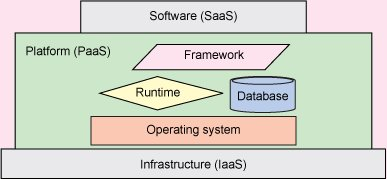
\includegraphics[width=8cm, keepaspectratio]{img/figure1.jpg}
			\label{fig_paas}
			\caption{Estrutura do PaaS}
		\end{figure}
		O que um bom provedor PaaS precisa ter:
			\begin{itemize}
		    \item Estrutura de desenvolvimento de aplicativo: Uma estrutura de desenvolvimento de aplicativo robusta desenvolvida em tecnologia amplamente usada, por exemplo, o Java;
            \item Disponibilidade: A plataforma de opção deve estar acessível e disponível em qualquer lugar, a qualquer hora;
            \item Escalabilidade: A plataforma deve ser inteligente o suficiente para aproveitar a capacidade elástica de uma infraestrutura;
            \item Segurança: Deve possuir dispositivos contra ataques;
            \item Inclusão: A plataforma deve fornecer a capacidade de incluir, embarcar e integrar outros aplicativos desenvolvidos nas mesmas plataformas ou em outras;
            \item Portabilidade: A plataforma deve permitir que as empresas movam o aplicativo de uma IaaS para outra.
		\end{itemize}
	\subsection{IaaS}
		Infraestrutura como Serviço (\textit{Infrastructure as a Service} (IaaS)) é a camada do \textit{Cloud Computer} de mais baixo nível. Ela pode ser defida como sendo a 'capacidade compucional' da nuvem. Ela é responsável pela infraestrura, ou seja, é nesta camada que se define a quantidade de processamento, de armazenamento, de memória RAM, etc. Toda esta estrutura pode ser encontrada em nossas casas, mas em escala muito menor. O IaaS trabalha nesse nicho, mas em escala industrial.
		
		O IaaS não é constituído por PCs(\textit{Personal Computer}), mas por diversos servidores robustos, e os dados ficam em \textit{storages}, que são máquinas que possuem grande contingência, poder de armazenamento e velocidade.
		
		Hoje em dia existem diversos serviços, que com apenas um clique pode se criar um servidor com a configuração que se deseja.
		
		O IaaS fornece seus serviços as outras duas camadas superiores, o PaaS e o SaaS.
		 
	\section{Possibilidades -- Soluções disponíveis no mercado}
		teste
	\section{Conclusão}
		teste
\end{document}
